\documentclass{article}
\usepackage{amsmath}
\usepackage{graphicx}
\usepackage{graphics}
\usepackage{amssymb}
\usepackage{booktabs}
\usepackage{listings}
\usepackage{color}
\usepackage{caption}
\usepackage{subcaption}
\usepackage[margin=0.8in]{geometry}

\definecolor{dkgreen}{rgb}{0,0.6,0}
\definecolor{gray}{rgb}{0.5,0.5,0.5}
\definecolor{mauve}{rgb}{0.58,0,0.82}

\begin{document}
\title{Homework 3 \\CS 5220}
\author{Lara Backer, Greg Granito, Sam Tung}

\maketitle

%%%%%%%%%%%%%%%%%%%%%%%%%%%%%%%%%%%%%%%%%%%%%%%%%%%%%%%%%%%%%%%%%%%%%%%
\section{Introduction}

This goal of this project is to optimize the parallelization of the Floyd-Warshall algorithm for finding the shortest path between two nodes in a graph. \\

A base parallelized C code using openMP was provided. From this, the objectives are to profile and tune the existing code, and to implement the parallelization of the algorithm using MPI.  

\section{OpenMP Code}

\subsection{Baseline Profiling}
A look into performance of the code was conducted by using Intel's VTUNE on Totient. Due to some technical issues with the cluster, we could not run the "advanced-hotspots" for profiling. 

	\begin{figure}[h!]
		\begin{center}
			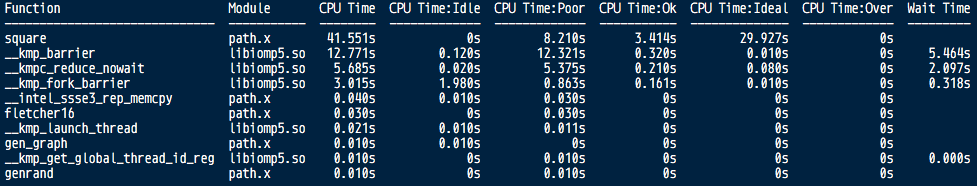
\includegraphics[width=0.7\columnwidth]{amplxe}
			\caption{Most time consuming functions in the base code.}
			\label{amplxe}
		\end{center}
	\end{figure}
	
From looking at VTUNE, it appears that the most time spent in the program was done on the square function which finds the minimum path between the nodes. This is not surprising, as there are plenty of nested for loops in the code, which undoubtedly takes a while to run through, as can be seen in Figure~\ref{square}.

\subsection{Vectorized Profiling}

One way to further increase the performance of the square function is to implement vectorization, which aligns data to promote efficiency. From the results, it appears that this does indeed increase performance slightly, as time in square is slightly less than it was previously. 

	\begin{figure}[h!]
		\begin{center}
			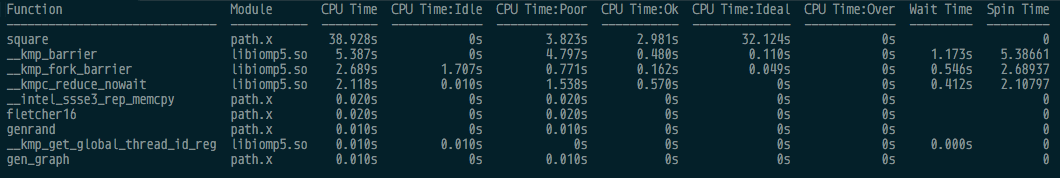
\includegraphics[width=.7\columnwidth]{amplxe_vector}
			\caption{OpenMP Code with vectorization.}
			\label{amplxe_vector}
		\end{center}
	\end{figure}
			
	
	\begin{figure}[h!]
		\begin{center}
			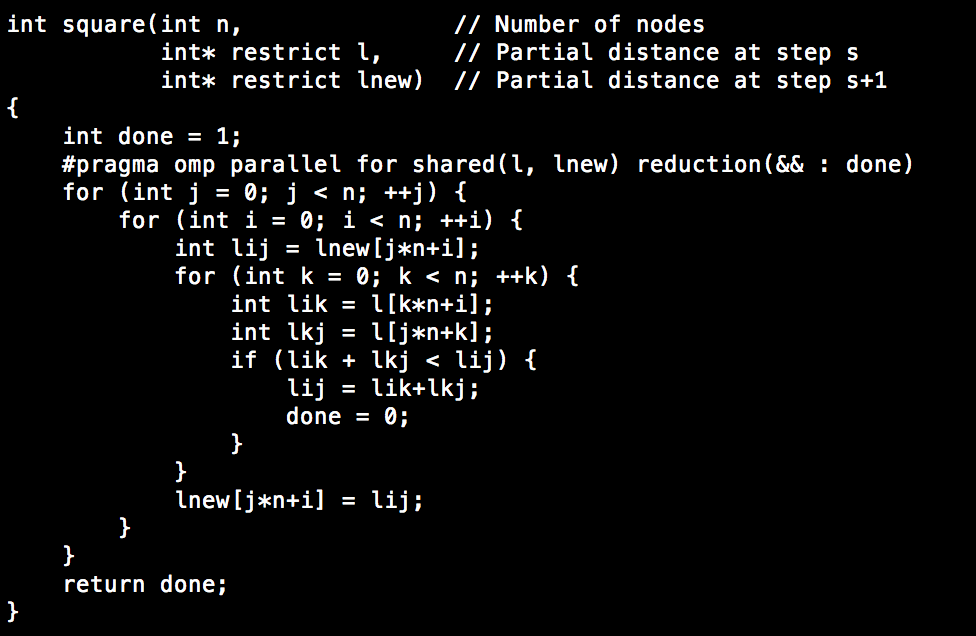
\includegraphics[width=0.5\columnwidth]{square}
			\caption{Square function}
			\label{square}
		\end{center}
	\end{figure}

\subsection{Scaling}
Strong scaling is defined as below, as the ratio of the time for a case to run in serial compared to a case with a given number of processors in parallel:
\begin{equation}
\textrm{Strong scaling} = \frac{t_{\textrm{serial}}}{t_{\textrm{parallel}}}
\end{equation}
Weak scaling is similarly defined as below as the ratio between serial and parallel case run times, although for weak scaling, the size of the computation on each processor is held constant. \\
\begin{equation}
\textrm{Weak scaling} = \frac{t_{\textrm{serial}}(n)}{t_{\textrm{parallel}}(n)}
\end{equation}

Both strong and weak scaling studies were performed for the openMP code.

	\begin{figure}[h!]
		\begin{center}
			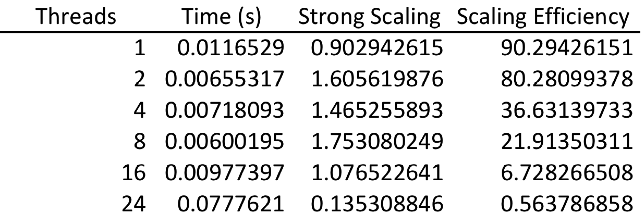
\includegraphics[width=0.5\columnwidth]{st_table_mp}
			\caption{Strong Scaling for 200x200 Element Graph, openMP}
			\label{mp_st_t}
		\end{center}
	\end{figure}
	
	\begin{figure}[h!]
		\begin{center}
			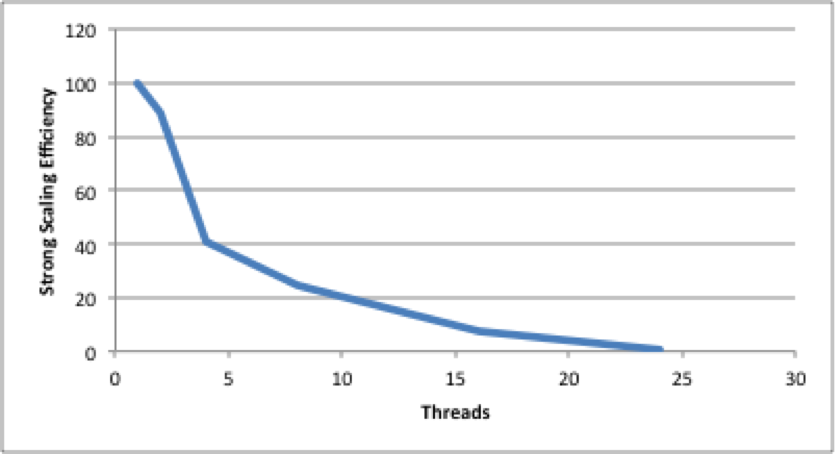
\includegraphics[width=0.7\columnwidth]{st_graph_mp}
			\caption{Strong Scaling Efficiency, openMP}
			\label{mp_st_g}
		\end{center}
	\end{figure}
	
	\begin{figure}[h!]
		\begin{center}
			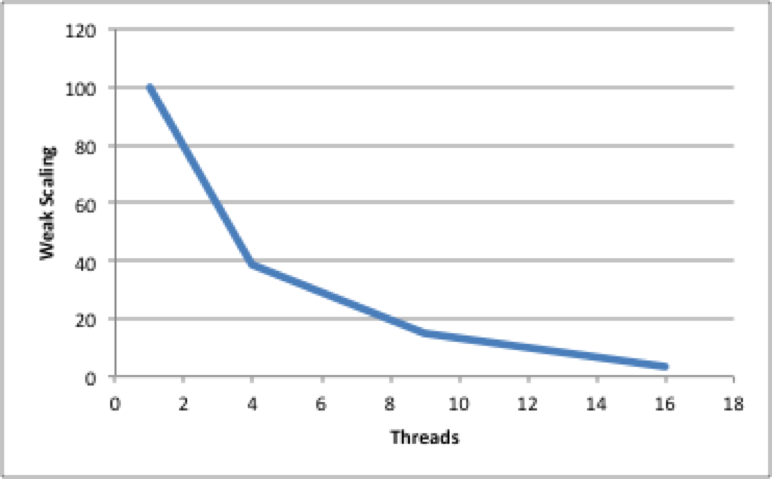
\includegraphics[width=0.7\columnwidth]{wk_graph_mp}
			\caption{Weak Scaling (\%), openMP}
			\label{wk_mp_g}
		\end{center}
	\end{figure}

\clearpage
\section{OpenMPI}

OpenMPI was used in place of OpenMP in the square routine to compare the efficiency of both methods. To use openMPI, the graph was split into equally sized sections, with each processor assigned a section. The minimum distance between locations within each section was computed, and then gathered and saved for the overall graph by using the command MPI\_ALLREDUCE and operation MPI\_MIN during the computation.  

\subsection{Profiling}
After attempting to implement OpenMPI, we once again look into performance of the code through profiling. 
	\begin{figure}[h!]
		\begin{center}
			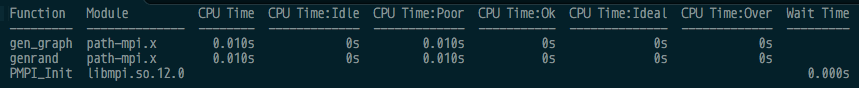
\includegraphics[width=0.7\columnwidth]{amplxe_mpi}
			\caption{Most time consuming functions in the OpenMPI implementation.}
			\label{amplxe_mpi}
		\end{center}
	\end{figure}

\subsection{Scaling}
Similarly, strong and weak scaling studies were performed with the MPI parallelization.

	\begin{figure}[h!]
		\begin{center}
			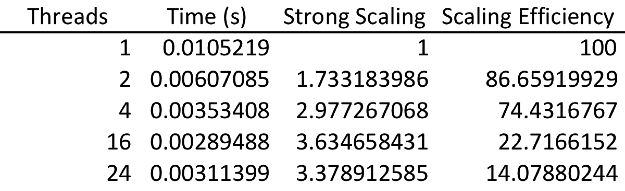
\includegraphics[width=0.5\columnwidth]{st_table_mpi}
			\caption{Strong Scaling for 200x200 Element Graph, openMPI}
			\label{st_mpi_t}
		\end{center}
	\end{figure}
	
	\begin{figure}[h!]
		\begin{center}
			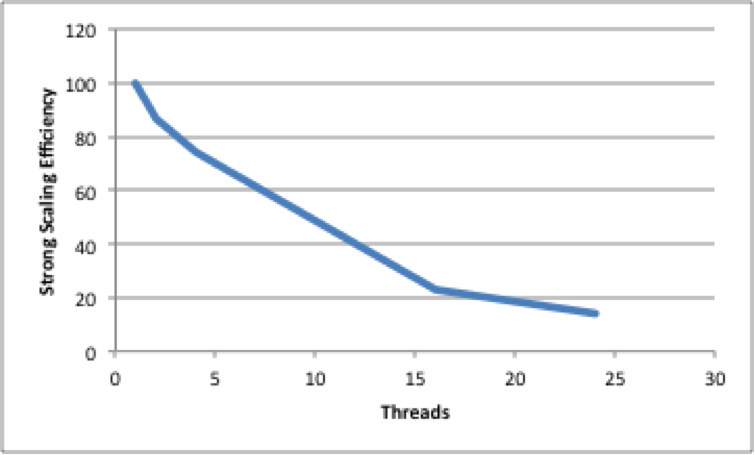
\includegraphics[width=0.7\columnwidth]{st_graph_mpi}
			\caption{Strong Scaling Efficiency, openMPI}
			\label{st_mpi_g}
		\end{center}
	\end{figure}
	
	\begin{figure}[h!]
		\begin{center}
			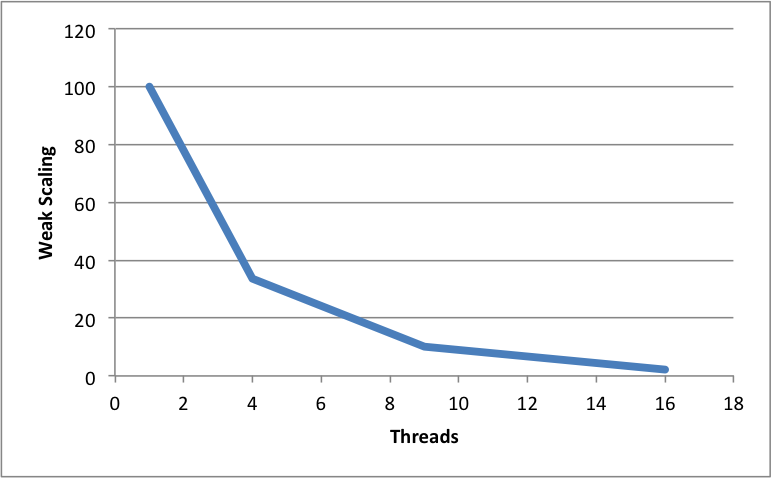
\includegraphics[width=0.7\columnwidth]{wk_graph_mpi}
			\caption{Weak Scaling (\%), openMPI}
			\label{wk_mpi_g}
		\end{center}
	\end{figure}
	
Overall, the current MPI parallelization method has better strong scaling than the openMP parallelization, although a similar domain decomposition for the openMP method would likely improve its' strong scaling characteristics. Weak scaling (which can be used to investigate the cost of communications) in both cases is similar, with openMPI performing only slightly more poorly. Additional testing should be done to investigate scaling on multiple nodes, in which case openMPI is expected to outperform openMP significantly due to the cross-node communications.  
	

\section{Additional Changes}
For the future, there are many different things we can try. As evidenced in the past, proper usage of compiler flags should be able to provide some speedups for the process. Additionally, another option we plan to try is blocking. On a conceptual level, for each block, the fastest paths would be calculated given each potential entry and exit point, which would be the ghost cells around each block. From there, one aggregated faster path through would be calculated from the combination of smaller paths. Finally, we hope to test the use of running the code on the Xeon Phis, for both the openMP and openMPI cases.

\end{document}